\documentclass[]{article}
\usepackage{atlasphysics}
% Nice maths macros
\usepackage{amsmath}
% Units
\usepackage{siunitx}
% Figures and floats
\usepackage{graphicx,subfigure,float}

% Graphics folider
\graphicspath{{figures/}}

% Scientific notation
% http://www.tapdancinggoats.com/easy-scientific-notation-in-latex.htm
\providecommand{\e}[1]{\ensuremath{\times 10^{#1}}}
% Differential Operator
\renewcommand{\d}[1]{\ensuremath{\,\operatorname{d}\!{#1}}}
% Absolute value
\renewcommand{\mod}[1]{\ensuremath{\lvert {#1} \rvert}}
% Airys functions Ai(x) and Bi(x)
\newcommand{\Ai}[1]{\ensuremath{\operatorname{Ai}({#1})}}
\newcommand{\Bi}[1]{\ensuremath{\operatorname{Bi}({#1})}}

\begin{document}

\title{Masses of S-State Quarkonium via the Roots of Airy's Function $\Ai{x}$}
\author{Alex Pearce}
\date{\today}
\maketitle


\begin{abstract}
We solve the Schr\"{o}dinger equation for $\ell = 0$ bound charm-anticharm \ccbar and bottom-antibottom \bbbar states in order to find the charm and bottom quark masses. The eigenvalues of the Hamiltonian may be found by finding the roots of Airy's functions $\Ai{x}$ and so a numerical approach, that of Ridder's method, was used to find these roots. The roots were then compared against experimentally obtained excited meson masses to find a charm mass of $m_{c} = 1.213\GeV$ and a bottom mass of $m_{b} = 4.505\GeV$. The linear radial potential $V = kr$ was found to differ slightly in strength for \ccbar and \bbbar with $\Delta k = TODO$.
\end{abstract}


\section{Introduction}\label{sec:intro}

A meson is a bound state of a quark and an antiquark. A neutral pion $\pi^{0}$, as an example, is a quantum superposition of \uubar and \ddbar, specifically $1/\sqrt{2}(\uubar + \ddbar)$. Quarkonia are a subset of the mesons, and are mesons comprised of a quark and its antiparticle \qqbar.\footnotemark\ A bound state of \ccbar is called charmonium and that of \bbbar is called bottomonium.

% Meson/Quarkonium distinction
\footnotetext{Note the distinction between a quark and \emph{any other} antiquark, such as $u\bar{s}$, and a quark and it's \emph{own antiparticle}, such as $\ccbar$. The latter is quarkonium, the former belongs in the broader category of mesons.}

Under the laws of QCD, we cannot observe states of colour; that is to say we can only see colourless states. Quarks and gluons (the gauge bosons of QCD) carry colour\footnotemark\ and hence cannot be observed on their own. This property of quarks and gluons is known as colour confinement. Because of colour confinement we cannot measure the quark mass directly and so must turn to indirect methods of measurement.

% Quark and gluon colour
\footnotetext{A quark carries one colour or anticolour such as red, green or antiblue ($r$, $g$ or $\bar{b}$) whilst a gluon carries a superposition of two one colour and one anticolour states such as red-antigreen and green-antired ($1/\sqrt{2}(r\bar{g} + g\bar{r})$). For an enlightening discussion on colour theory see Griffiths~\cite{ref:dgriffithsparticles}.}

As all mesons are colourless they are, in principle, observable. (They may decay extremely quickly or be very massive making them difficult to produce and/or observe, however.) We may nav\"{i}ely think that if we can measure the masses several different mesons then we could extract the constituent quark masses from the data, but the mass of meson is not just the sum of the `bare masses' of the quarks inside; it is this bare mass plus the binding energy between the two quarks. This leads us to conclude that if we could obtain the binding energy then we could obtain the individual quark masses.

TODO: put sections numbers in the bit below

We set out by solving the Schr\"{o}dinger equation for quarkonium to find that it's solution is Airy's function $\Ai{x}$, where the roots of this function are related to the binding energy of the \qqbar pair.

We find the roots via a numerical algorithm and then plot these roots against experimental data of meson masses in order to extract both the strength of the binding potential $V=kr$ and the charm and bottom quark masses $m_{c}$ and $m_{b}$.


\section{Solving the Schr\"{o}dinger equation for \qqbar}\label{sec:schrodinger}

We start by presuming that the bound \qqbar meson is massive enough such that we may use non-relativistic quantum mechanics, hence we employ the Schr\"{o}dinger equation. TODO: Why? We solve the time-independent radial equation (cf.\ the Hydrogen atom~\cite{ref:dgriffithsquantum})
\begin{equation}\label{eqn:schrodinger}
-\frac{\hbar^{2}}{2m}\left (
	\frac{1}{r^{2}} \frac{\d{}}{\d{r}} \left (
		r^{2} \frac{\d{\psi}}{\d{r}}
	\right )
	- \frac{\ell(\ell+1)}{r^{2}}\psi
\right )
+ V(r)\psi = E\psi.
\end{equation}
Here $m$ is the so-called reduced mass (equal to half of each constituent quark mass e.g. $m_{c}/2$ for charmonium), $\ell$ is the orbital angular momentum quantum number, $V(r)$ is the binding potential, $\psi$ is the eigenwavefunction of the Hamiltonian $H$ and $E$ is the eigenvalue for $\phi$ under $H$. Note this is, as mentioned, an eigenvalue problem $H\psi=E\psi$.

\subsection{Assumptions}\label{ssec:assumptions}

We shall investigate quarkonium states with zero angular momentum, that is $\ell = 0$. In addition, as mentioned previously, we shall work in the non-relativistic regime.

The most crucial approximation that we make is that of the binding potential $V(r)$. We shall use a linear potential model $V(r) = kr$ where $k$ is some real coefficient. The value of $k$ is not known but may be deduced using the relation between meson mass and quark mass as follows.

As stated previously, we anticipate that the measured mass of meson is not only the mass of its constituent quarks but also the binding energy of the bound system (via the mass-energy equivalence $E=mc^{2}$). Then, we assume a measured meson mass conforms to
\begin{equation}\label{eqn:mesonmass}
M_{n} = 2m_{q} + E_{n}
\end{equation}
where $n$ refers to the $n$th \emph{excited state} of the meson~\cite{ref:buchmuller}. The excited states may be thought of like those of an electron orbiting a proton: the bound quarks may occupy infinitely many quantised energy levels of increasing radial distance and increasing energy. It follows that equation \ref{eqn:mesonmass} represents the quarkonium \emph{spectrum}.

Given experimental data of excited meson masses then, we can plot our binding energies $E_{n}$ against them to find the quark mass $m_{q}$.

\subsection{Manipulation}

We may work our Schr\"{o}dinger equation in to a much more manageable form. First, we apply our $\ell = 0$ assumption and make the change of variable $u = r\psi$
\[
-\frac{\hbar^{2}}{2m}
 \frac{\d{^{2}u}}{\d{r}^{2}}
+ V(r)u = Eu.
\]
After moving the $Eu$ over to the left and making one further change of variable $r = ax + b$ we  arrive at
\begin{equation}\label{eqn:airys}
\frac{\d{u}}{\d{x}} - xu = 0,
\end{equation}
where we have chosen $a = \sqrt[3]{2mk/\hbar^{2}}$ and $b = E/k$.

This is beneficial is several ways. Not only has the problem been reduced to a single order ordinary differential equation (ODE), the ODE is a well studied one that is analytically solvable. In particular, equation \ref{eqn:airys} is Airy's equation with solutions $y(x) = c\Ai{x} + d\Bi{x}$. The two solutions $\Ai{x}$ and $\Bi{x}$ are known as Airy's function. We note that as $\Bi{x}$ becomes singular as $x$ tends to infinity it is a non-physical solution and so $d = 0$. This leaves us with $\Ai{x}$ (referred to from now on as `Airy's function') as the solution to our ODE.\footnotemark
\[
y(x) = \Ai{x}
\]

\footnotetext{$\Ai{x} \to 0$ as $x \to \pm\infty$.}

\section{Approximation of \Ai{x}}\label{sec:approximation}

We require that as $r \to 0$ our wavefunction $\psi$ remains finite. As $u = r\psi$, it follows that $u \to 0$ as $r \to 0$. We must now require that $\Ai{x = 0} = 0$, i.e.\ we need to find to roots of Airy's function. As $r = ax + b$, the $n$th root of Airy's function corresponds to
\begin{equation}\label{eqn:rootexpression}
\Ai{x} = 0 \quad\Rightarrow\quad x_{n} = -\frac{b}{a} = -E_{n}\sqrt[3]{\frac{\hbar^{2}}{2mk^{4}}}
\end{equation}

In order to do this we shall approximate Airy's function with three different representations. This is often necessary for analytical functions that vary there form along $x$, e.g.\ changing from oscillatory to exponential, hence different expansions are favoured for different ranges in $x$.

The three approximations for Airy's function $\Ai{x}$ are given here without a full explanation of terms, but are reproduced in full in appendix \ref{app:approximations}.

For small $\mod{x}$ we have~\cite{ref:abramowitz}

\begin{equation}\label{eqn:airyfirst}
\Ai{x} = 0.3550280538f(x) - 0.2588194037g(x),
\end{equation}

For larger $\mod{x}$ we may use the alternative approximations
\begin{align}\label{eqn:airysecond}
\Ai{x} \approx \frac{1}{2}\pi^{-1/2}x^{-1/4}e^{-\zeta} \sum\limits_{k=0} (-1)^{k}c_{k}\zeta^{-k},
\end{align}
and
\begin{equation}\label{eqn:airythird}
	\begin{split}
		\Ai{-x} \approx \pi^{-1/2}x^{-1/4}
		\Bigl(
			&\sin{(\zeta + \frac{\pi}{4})}\sum\limits_{k=0}(-1)^{k}c_{2k}\zeta^{-2k} -\\
			&\cos{(\zeta + \frac{\pi}{4})}\sum\limits_{k=0}(-1)^{k}c_{2k+1}\zeta^{-(2k+1)}
		\Bigr),
	\end{split}
\end{equation}

Equations \ref{eqn:airysecond} and \ref{eqn:airythird} are the Chebyshev expansions of Airy's function $\Ai{x}$~\cite{ref:agil}. The coefficients $c_{k}$ (see equation \ref{eqn:ck}) are in fact divergent, but the series expansions give good approximations up to around $k = 5$.

We will refer to equations \ref{eqn:airyfirst}, \ref{eqn:airysecond}, and \ref{eqn:airythird} and the first, second, and third approximation of Airy's function respectively (keeping in mind that each representation is appropriate for different values of $x$).

A comparison of the different approximations is given in figure \ref{fig:approximations}. The data has been presented in such a way so as to illustrate how each approximations diverges outside a given range of $x$.

The first approximation gives satisfactory result for approximately $-13 < x < 7$, the second for $x > 5$, and the third for $x < -4$. Clearly the roots of \Ai{x} are all negative, hence we shall not need the second approximation.

We shall then use a combination of the first and third approximations, specifically the first for $-8 < x < 0$ and the third for $x < -8$.

\subsection{Recursive Computation}\label{ssec:recursion}

The expressions for the series expansions coefficients $c_{k}$ in equation \ref{eqn:ck} are clearly quite cumbersome, but we may tame them to a degree via recursive computation. The functions $f(x)$ and $g(x)$ in the first approximation of $\Ai{x}$ may also be treated recursively (see equations \ref{eqn:airyfirstf} and \ref{eqn:airyfirstg}).

The advantages of recursive computation are many, but for our purposes they allow us to compute moderately small numbers that may involve large terms during computation.

For example, $f(x)$, as in equation \ref{eqn:airyfirstf}, carries a factorial in the denominator of each term. The factorial function $n!$ grows extremely rapidly with $n$,\footnotemark~ but if we note that each factorial term is simply $(n+3)!$, where $n$ is the factorial argument of the \emph{previous} term, all we have to do to find the next term is multiply the previous term by $(n+1)(n+2)(n+3)$.

\footnotetext{Interestingly, the factorial $n!$ grows even faster than the exponential function $e^{n}$.}

As the factorial is in the denominator, the final number will be small, but computing this by blindly calculating $x!$ will result in storing huge numbers in memory as the number of terms in the series increases. Modern computers can only handle numbers of a certain magnitude before they overflow, causing large numerical errors. Recursion stops the storage of large numbers in memory, preventing this problem.

The derivation of the recursive forms of $f(x)$, $g(x)$, and the coefficients $c_{k}$ are given in appendix \ref{app:recursion}. Note that $c_{k}$ in particular benefits from recursive computation as it prevents us having to calculate $216^{k}$, only requiring us to multiply successive terms by $1/216$ (which is also much less expensive computationally). TODO: mention how many terms the recursive term can handle vs. the regular computation.

\subsection{Roots of \Ai{x}}

We have now reduced the task of solving the Schr\"{o}dinger equation (equation \ref{eqn:schrodinger}) to numerically approximating and then finding the roots of Airy's function.

By inspecting figure \ref{fig:approximations}, we see that the first root occurs just after $x = 2$. In order to find the roots then, we shall `walk' along the function until the sign changes, in which case we know there is a root between the previous and current step $x_{n-1}$ and $x_{n}$.

This root finding algorithm is extremely simple, and quite useless in that it cannot converge. We may decrease the step size of the walk in order to add more precision to the bracketed root, but we still wouldn't have a number for the root (only two numbers which contain the root) nor would we have good performance (we would waste time walking along the parts of function without roots).

To remedy this, we shall use our walking procedure to find the bracketed roots, and then pass the bracket values to a numerical algorithm called Ridder's method~\cite{ref:nr}. Ridder's method accepts two values $x_{1}$ and $x_{2}$ for which $\Ai{x_{1} < x_{R} < x_{2}} = 0$ for some $x_{R}$, a root of Airy's function. It then iteratively finds the root of a function to a desired precision.

Ridder's method quick to converge and nicely allows us to provide a precision. A small selection of other root finding algorithms along with Ridder's method are compared in section \ref{sec:algorithms}.

Once we have obtained the roots, the energy of the $n$th excited state of quarkonium may be found from equation \ref{eqn:rootexpression}
\begin{equation}
E_{n} = -x_{n} \sqrt[3]{\frac{2mk^{4}}{\hbar^{2}}}
\end{equation}

\section{Results}\label{sec:results}

The roots of Airy's function as found by Ridder's method are given in table \ref{tab:roots}.   Ridder's method was passed a precision of $\num{e-10}$. It is clear that our computed roots $x_{n}^{\mathrm{comp}}$ match extremely well with the reference roots~\cite{ref:abramowitz}, in fact matching with the precision passed this Ridder's method.

This excellent agreement shows that the representations of \Ai{x} in equations \ref{eqn:airyfirst} and \ref{eqn:airythird} must give very accurate and precise approximations. The difference between the computeted and reference roots $\Delta x_{n} = x_{n}^{\mathrm{comp}} - x_{n}^{\mathrm{ref}}$ is of the order $\num{e-10}$, which is exactly the precision we told Ridder's method to use. It is a reasonable assumption that the approximations of Airy's function we used are capable of even more precision if desired.\footnotemark

\footnotetext{The use of a precision of $\num{e-10}$ was twofold: the reference roots $x_{n}^{\mathrm{ref}}$ were given up to ten decimal places making comparison difficult, and the meson masses with which we compare the roots are given to three decimal places. Hence a precision larger than $\num{e-10}$ would have been superfluous.}

Given the experimental mesons masses in table \ref{tab:mesonmasses}~\cite{ref:gdaniell}, the computed roots were plotted against these masses. The resulting plot is shown in figure \ref{fig:data}.

Despite a limited data set for the Charmonium masses, both sets of plotted points indicate a linear relationship, which supports our use of a liner potential. Via equation \ref{eqn:mesonmass}, the intercept of the superimposed lines gives twice the quark mass $m_{q}$, whilst the slopes allow us to calculate $k$. Using this we present
\begin{align*}
m_{c} = 1.21\GeV&,\quad m_{b} = 4.51\GeV,\\
k_{c} = \num{3.11e11}\si{\joule\per\metre}&,\quad k_{b} = \num{4.08e11}\si{\joule\per\metre}.
\end{align*}

The above data presumes absolute accuracy in the experimental data~\cite{ref:gdaniell} used. Without errors on the experimental meson masses it is difficult to provide meaningful errors with our results.

\subsection{Comparison}

Data does exist for the charm and bottom quark masses~\cite{ref:pdg}, giving $m_{c} = 1.29^{+0.05}_{-0.11}\GeV$ and $m_{b} = 4.67^{+0.18}_{-0.06}\GeV$.\footnotemark

\footnotetext{We have used the 1S scheme for the bottom mass as it more appropriate for our low-energy regime.}

These agree quite well with our data, differing by $7\%$ for the charm and $4\%$ for the bottom quark. In both cases our data gives a slightly higher quark mass.

We postulate that the difference in mass is due to two main factors. Firstly, the experimental data used was of unknown source and was without errors, forbidding research on them and meaningful errors on our own data. Secondly, the simple form of the binding potential $V(r)$ is unlikely to represent the true QCD binding potential. A better fit to other data may have been achieved with another potential such as the Cornell potential~\cite{ref:eichten}
\[
V(r) = \frac{a}{r} + br,
\]
or other, more complex, candidates.

It is worthy of note however just how far the simple linear potential has bought us and also how well the Airy function approximations used performed.

\section{Root Finding Algorithms}

TODO: this.

\section{Conclusions}

TODO: this.

\section{Tables}

\begin{table}[H]
	\begin{center}
		\begin{tabular}{ c c c }
			$n$ & $x_{n}^{\mathrm{comp}}$ & $x_{n}^{\mathrm{ref}}$\\
			\hline
			1  & -2.3381074104  & -2.3381074101 \\
			2  & -4.0879494441  & -4.0879494438 \\
			3  & -5.5205598280  & -5.5205598278 \\
			4  & -6.7867080900  & -6.7867080898 \\
			5  & -7.9441335871  & -7.9441335869 \\
			6  & -9.0226508533  & -9.0226508531 \\
			7  & -10.0401743416 & -10.0401743414\\
			8  & -11.0085243037 & -11.0085243036\\
			9  & -11.9360155632 & -11.9360155631\\
			10 & -12.8287767529 & -12.8287767527
		\end{tabular}
		\caption{Roots of \Ai{x}. Computed are $x_{n}^{\mathrm{comp}}$, the reference roots~\cite{ref:abramowitz} are $x_{n}^{\mathrm{ref}}$. The difference between the two is $\Delta x_{n} = x_{n}^{\mathrm{comp}} - x_{n}^{\mathrm{ref}} \sim \num{e-10}$ for all roots.}
		\label{tab:roots}
	\end{center}
\end{table}

\begin{table}[H]
	\begin{center}
		\begin{tabular}{ c c c c }
			$n$ & \ccbar & & \bbbar\\
			\hline
			1 & 3.10 & & 9.46 \\
			2 & 3.69 & & 10.02\\
			3 & 4.04 & & 10.35\\
			4 &      & & 10.57\\
			5 &      & & 10.86\\
			6 &      & & 11.02\\
		\end{tabular}
		\caption{Quarkonium masses with $\ell = 0$ in \GeV~\cite{ref:gdaniell}.}
		\label{tab:mesonmasses}
	\end{center}  
\end{table}

\section{Root Finding Algorithms}\label{sec:algorithms}


\section{Figures}\label{sec:figures}

\begin{figure}[H]
	\hspace*{-0.15\textwidth}
	\centering
	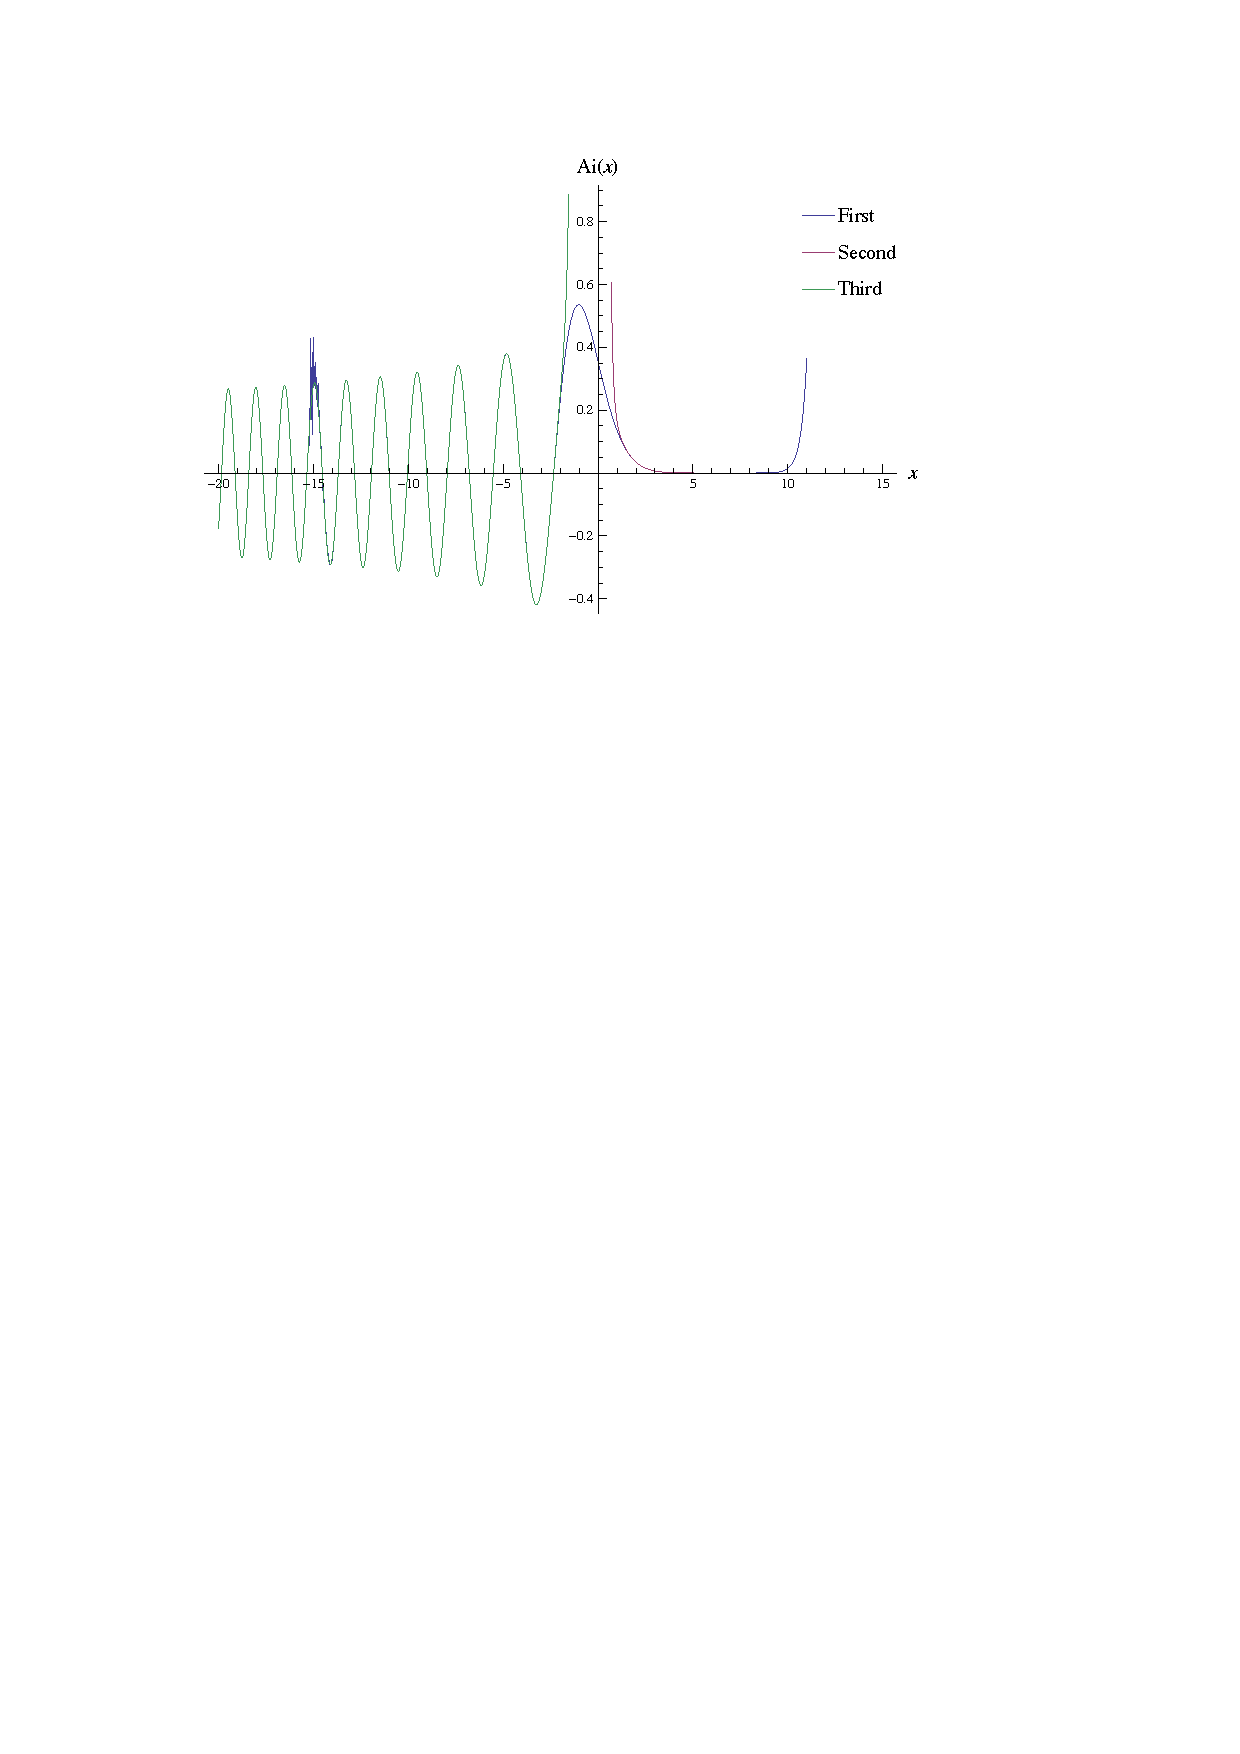
\includegraphics[scale=1.3]{approximations}
	\caption{The first, second, and third approximations of \Ai{x} as given in equations \ref{eqn:airyfirst}, \ref{eqn:airysecond}, and \ref{eqn:airythird} respectively.}
	\label{fig:approximations}
\end{figure}

\begin{figure}[H]
	\hspace*{-0.15\textwidth}
	\centering
	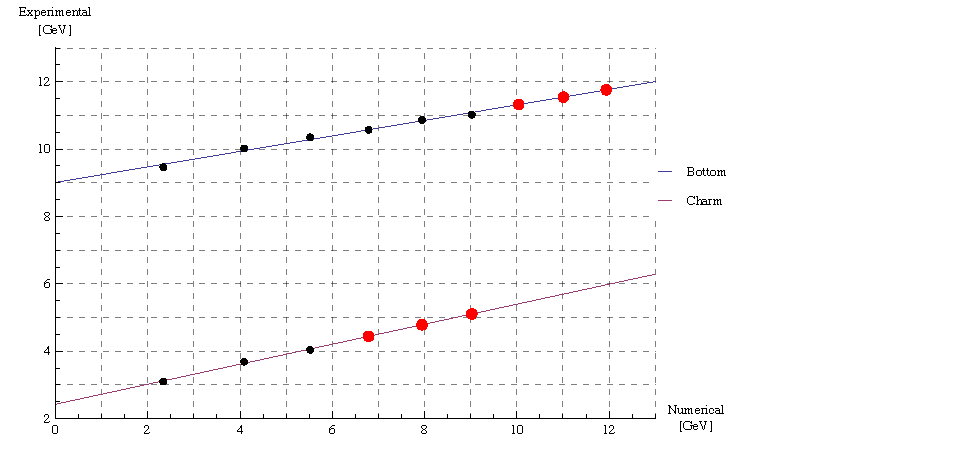
\includegraphics[scale=1.3]{experimental-numerical}
	\caption{TODO: Caption here}
	\label{fig:data}
\end{figure}


\appendix
\section{Approximations of \Ai{x}}\label{app:approximations}

For small $\mod{x}$ we have

\[\Ai{x} = 0.3550280538f(x) - 0.2588194037g(x),\]
where $f(x)$ and $g(x)$ are infinite series given by
\begin{align}
f(x) &= 1 + \frac{1}{3!}x^{3} + \frac{1\times4}{6!}x^{6} + \frac{1\times4\times{7}}{9!}x^{9} + \dotsb,\label{eqn:airyfirstf}\\
g(x) &= x + \frac{2}{4!}x^{4} + \frac{2\times5}{7!}x^{7} + \frac{2\times5\times{8}}{10!}x^{10} + \dotsb\label{eqn:airyfirstg}.
\end{align}

For larger $\mod{x}$ we may use the alternative approximations
\[
\Ai{x} \approx \frac{1}{2}\pi^{-1/2}x^{-1/4}e^{-\zeta} \sum\limits_{k=0} (-1)^{k}c_{k}\zeta^{-k},
\]
and
\[
	\begin{split}
		\Ai{-x} \approx \pi^{-1/2}x^{-1/4}
		\Bigl(
			&\sin{(\zeta + \frac{\pi}{4})}\sum\limits_{k=0}(-1)^{k}c_{2k}\zeta^{-2k} -\\
			&\cos{(\zeta + \frac{\pi}{4})}\sum\limits_{k=0}(-1)^{k}c_{2k+1}\zeta^{-(2k+1)}
		\Bigr),
	\end{split}
\]
where
\begin{equation}\label{eqn:ck}
c_{k} = \frac{(2k+1)(2k+3)\dotsb(6k-1)}{216^{k}k!} = 1,
\end{equation}
with $c_{0} = 1$. Lastly
\[
\zeta = \frac{2}{3}x^{3/2}.
\]

\subsection{Recursive Representation}\label{app:recursion}

After some algebra, the functions $f(x)$ and $g(x)$ in the first approximation of $\Ai{x}$ may be represented recursively. The $n$th term in each series are then
\begin{align*}
f_{n}(x) &= \frac{f_{n-1}(x)}{(3n^{2} - n)} \frac{x^{3}}{3},\\ 
g_{n}(x) &= \frac{g_{n-1}(x)}{(3n^{2} + n)} \frac{x^{3}}{3},
\end{align*}
where $f_{0}(x) = 1$ and $g_{0}(x) = x$.

The series coefficients $c_{k}$ used in the second and third approximations of $\Ai{x}$ may also be presented recursively.
\[
c_{k} = c_{k-1} \frac{(6k-5)(6k-3)(6k-1)}{216k(2n-1)}
\]
where $c_{0} = 1$.

% Woo Bibtex!
\bibliographystyle{IEEE}
\bibliography{bibliography}

\end{document}